
\chapter{DISEÑO CONCEPTUAL ESTRUCTURAL}







\section{Cumplimiento de la especificación \\proporcionada.} % section headings are printed smaller than chapter names

\begin{figure}[h]
  \centering
    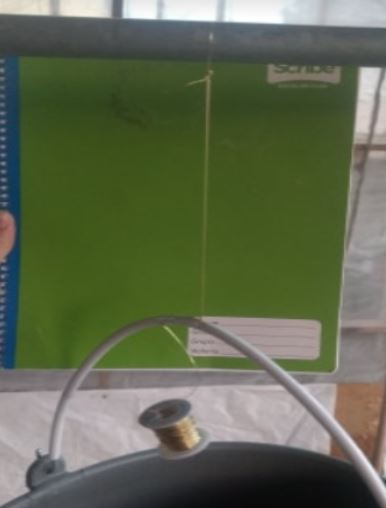
\includegraphics[width=\textwidth]{A/figs/A_1.jpg}  
    \caption{Superior} % should be 1.1
\end{figure}

\begin{figure}[h]
  \centering
    \includegraphics[width=\textwidth]{A/figs/A_2.jpg}  
    \caption{Inferior} % should be 2.1 - actually is 2 or 2.2 with optional code
\end{figure}
\ \ \ 
\section{Planos descriptivos de fabricación y ensamble.}



\begin{center}
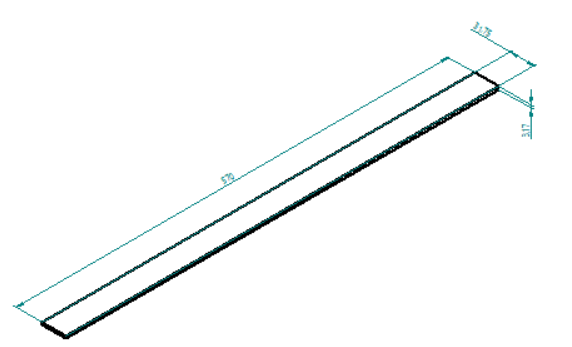
\includegraphics[width=.6\linewidth]{A/figs/B_1.png} 
 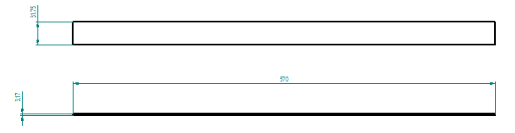
\includegraphics[width=.6\linewidth]{A/figs/B_2.png} 

\end{center}

\begin{center}
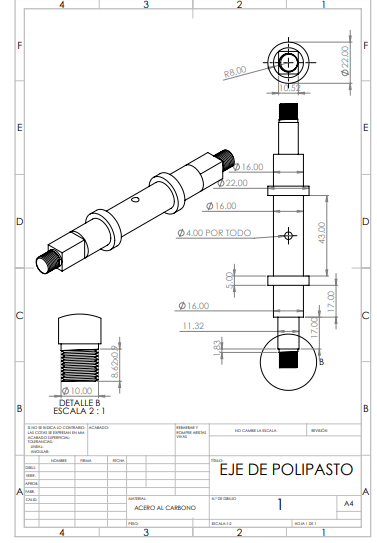
\includegraphics[width=1\linewidth]{A/figs/C_1.png} 
\end{center}

\begin{center}
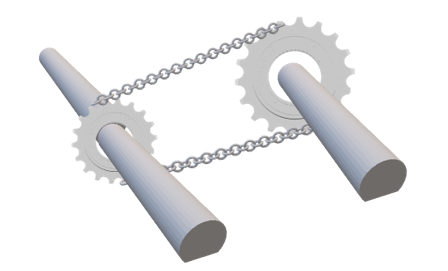
\includegraphics[width=.6\linewidth]{A/figs/C_2.png} 
\end{center}

\begin{center}
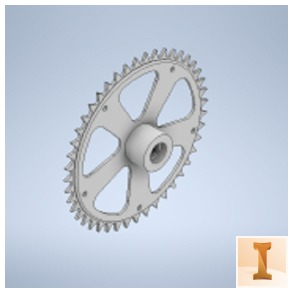
\includegraphics[width=.6\linewidth]{A/figs/elements/A_5.jpeg} 
 

\end{center}

\begin{center}
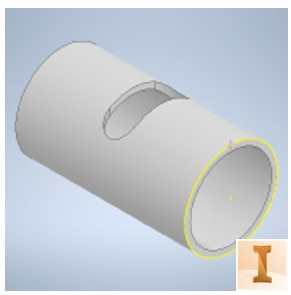
\includegraphics[width=.3\linewidth]{A/figs/elements/A_1.jpeg}  
\includegraphics[width=.3\linewidth]{A/figs/elements/A_2.jpeg}  
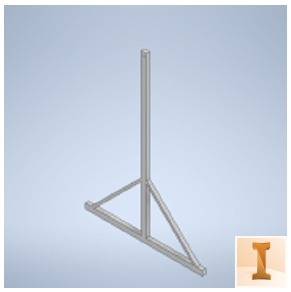
\includegraphics[width=.3\linewidth]{A/figs/elements/A_3.jpeg}
\\[\baselineskip]% adds vertical line spacing
\quad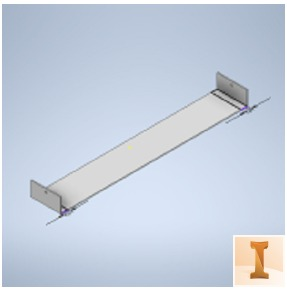
\includegraphics[width=.3\linewidth]{A/figs/elements/A_4.jpeg}  
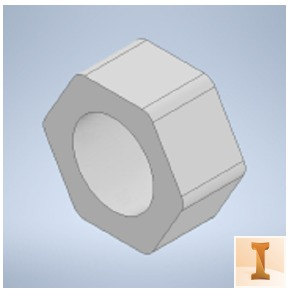
\includegraphics[width=.3\linewidth]{A/figs/elements/A_7.jpeg} 
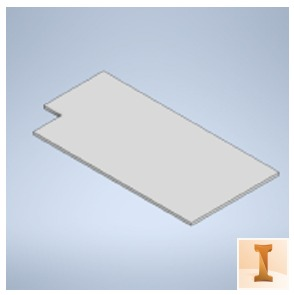
\includegraphics[width=.3\linewidth]{A/figs/elements/A_6.jpeg} 

\end{center}



\begin{center}
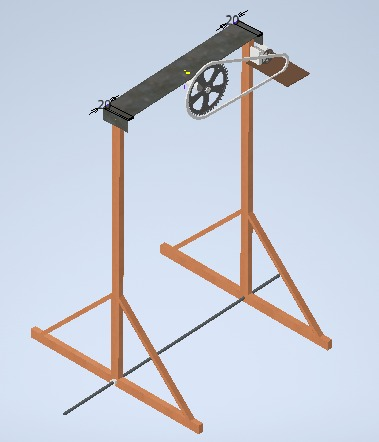
\includegraphics[width=.6\linewidth]{A/figs/elements/A_8.jpeg}  
\end{center}

\begin{center}
\quad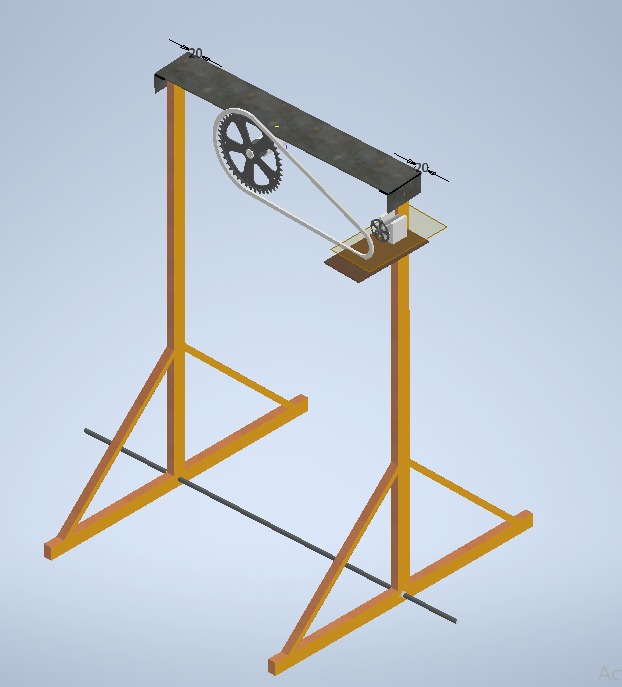
\includegraphics[width=1\linewidth]{A/figs/elements/A_9.jpeg}  


\end{center}
